%%=============================================================================
%% Inleiding
%%=============================================================================

\chapter{\IfLanguageName{dutch}{Inleiding}{Introduction}}%
\label{ch:inleiding}

% inleiding taal en onderwijs
Het middelbaar onderwijs staat op springen. Dagelijks sneuvelen leerkrachten en scholieren van het middelbaar onderwijs onder de te harde werkdruk \autocite{Glorieux2018}. Lezen is ingebed in ons dagelijks leven in de vorm van Nederlandstalige nieuwsartikelen tot de ondertiteling van televisieseries. Mensen van eender welke leeftijdsgroep kunnen lezen niet ontsnappen en dit moet van jongs af aan geprikkeld worden \autocite{Daoud2023}.

\subsubsection{Vakmiddelen -en didactiek in het onderwijs}
Lerarenopleidingen benadrukken nu het gebruik van verschillende bronnen in lessen. De leesgraad van deze bronnen verandert echter niet, want de noodzaak aan bronnen met diverse leesgraden is bedoeld om scholieren uit te kunnen dagen \autocite{Surma2019}. Het Amerikaanse onderwijs stampte C.R.E.A.T.E.\footnote{https://teachcreate.org/} uit de grond. Dit initiatief zet scholieren tussen 12 en 18 jaar aan om wetenschappelijke artikelen te lezen in plaats van enkel boeken. Scholieren komen zo in direct contact met wetenschappelijk onderzoek. Ze begrijpen hoe wetenschappers experimenten uitvoeren, plannen en resultaten analyseren en interpreteren. Vlaamse STEM-leerkrachten in de derde graad middelbaar onderwijs moeten volgens het M-decreet en de leerplannen van zowel het katholiek\footnote{https://pro.katholiekonderwijs.vlaanderen/basisoptie-stem/ondersteunend-materiaal} als het gemeenschapsonderwijs\footnote{https://g-o.be/stem/} hun theorielessen op een toegankelijke manier aanbieden, zodat alle scholieren worden meegenomen in het verhaal. 

\subsubsection{Kunstmatige intelligentie in Vlaanderen}
België is met een jaarlijks budget van 32 miljoen een pionier op het gebied van artificiële intelligentie (AI) op de werkvloer \autocite{Crevits2022}. Zo stampte de Vlaamse overheid verschillende AI-projecten uit de grond, om Vlaamse AI-ontwikkelingen te ondersteunen en om AI-softwarebedrijven te inspireren. Het amai!-project\footnote{https://amai.vlaanderen/} brengt AI-softwarebedrijven uit diverse domeinen samen en leidt tot het ontstaan van AI-toepassingen die processen automatiseren en de werkdruk verminderen, zoals real-time ondertiteling in de klas en een taalassistent voor leerkrachten in meertalige klasgroepen.

\section{\IfLanguageName{dutch}{Probleemstelling}{Problem Statement}}%
\label{sec:probleemstelling}

Vlaamse en Nederlandse onderzoeken van \textcite{Wentink2008, Desoete2017} wijzen uit dat gemiddeld 4\% van de Vlaamse en Nederlandse bevolking de diagnose van dyslexie heeft. Het aantal scholieren met dyslexie in het lager en middelbaar onderwijs wereldwijd loopt op tot 15\% ingeschat \autocite{Bonte2020, VanDerMeer2022}. \textcite{Lissens2020} benadrukt dat de impact van leerstoornissen niet stopt na het middelbaar onderwijs. Scholieren met dyslexie in het middelbaar onderwijs kampen met unieke uitdagingen, waaronder een moeizame en stroeve automatisering bij het lezen en spellen. Deze doelgroep kunnen rekenen op ondersteuning van coaches en beschikbare hulpmiddelen om hun leesachterstand te beperken. Het leerplan voor STEM-vakken stimuleert het gebruik van wetenschappelijke artikelen, maar houdt niet altijd rekening met de complexe leesgraad. De ingewikkelde woordenschat en syntax in wetenschappelijke artikelen kunnen een hindernis vormen voor de begrijpelijkheid van een tekst, waardoor scholieren met dyslexie de kerninhoud moeilijk kunnen doorgronden. Teksten vereenvoudigen, zonder de kern- en bijzaken te verliezen, kan een oplossing bieden. 

Leesvaardigheid is cruciaal voor succes op school en in het werkveld. Mensen met dyslexie kunnen problemen hebben met spelling, wat kan leiden tot onzekerheid en stress. Vooroordelen zijn nog steeds een probleem en kunnen leiden tot stigmatisering. Onderzoek toont echter aan dat mensen met dyslexie doorzettingsvermogen hebben en goede probleemoplossers zijn \autocite{Ghesquiere2018, Lissens2020, Bonte2020}. Ondersteuning op scholen en werkplekken is belangrijk, omdat dyslexie uitdagingen kan veroorzaken bij het betreden van de arbeidsmarkt. Onderzoek richt zich vooral op kinderen, maar ook jongvolwassenen en ouderen hebben ondersteuning nodig. Een gepersonaliseerde analyse is nodig om specifieke begeleiding te kunnen bieden bij begrijpend lezen \autocite{VanVreckem2015, Lissens2020}. De driejaarlijkse PISA-test meet de wiskundige en wetenschappelijke geletterdheid van 15-jarigen in ongeveer 79 geïndustrialiseerde landen. In 2018 namen 4822 Vlaamse scholieren van vijftien jaar deel aan deze test. Hoewel leer- en leesstoornissen niet worden meegenomen in de test, geven de resultaten een idee van de leesvaardigheid en wetenschappelijke geletterdheid van scholieren van die leeftijd. 

\begin{figure}[H]
	\begin{center}
		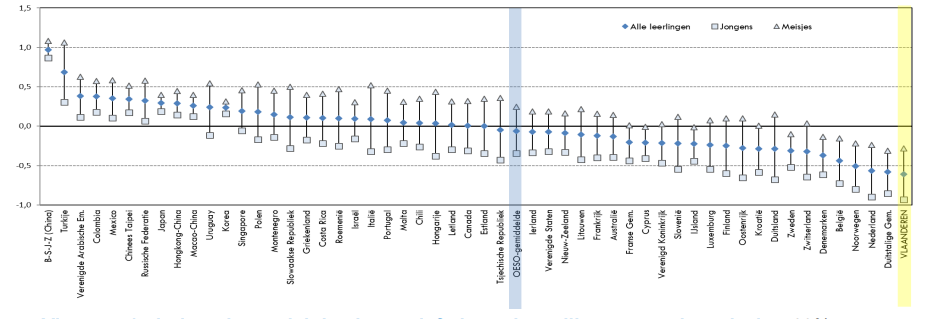
\includegraphics[width=\linewidth]{img/oeso-graphic-leesplezier.png}
	\end{center}
	\caption{Figuur van \textcite{DeMeyer2019}. Het leesplezier van Vlaamse 15-jarigen. Zij uitten zich uiterst negatief op stellingen over leesplezier. Volgens de enquète vond de helft van de scholieren begrijpend lezen enkel tijdsverlies en slechts 17\% gaf aan dat lezen één van hun favoriete hobby's is. Er is wel een significant verschil tussen de mening van jongens en meisjes, waar jongens negatiever antwoorden op lezen.}
\end{figure}

Wetenschappelijke artikelen vereenvoudigen kan tijd en energie van docenten in de derde graad middelbaar onderwijs opslorpen. Het Vlaamse middelbaar onderwijs staat onder druk en docenten hebben moeite om met deze werkdruk boven water te blijven. Daarom is er nood aan software die wetenschappelijke artikelen automatisch kan vereenvoudigen, specifiek gericht op de unieke noden van scholieren met dyslexie. Een dergelijke toepassing kan scholieren met dyslexie in de derde graad middelbare onderwijs ondersteunen bij het lezen van een wetenschappelijk artikel en kan het routinematige werk van STEM-docenten verminderen. 

\section{\IfLanguageName{dutch}{Onderzoeksvraag}{Research question}}%
\label{sec:onderzoeksvraag}

De volgende onderzoeksvraag is opgesteld: ”Hoe kan een wetenschappelijke artikel automatisch vereenvoudigd worden, gericht op de unieke noden van scholieren met dyslexie in de derde graad middelbaar onderwijs?”. Daarnaast worden de volgende deelvragen beantwoord.

\begin{itemize}
	\item Welke aanpakken zijn er voor geautomatiseerde tekstvereenvoudiging? Aansluitende vraag: "Hoe worden teksten handmatig vereenvoudigd voor scholieren met dyslexie?"
	\item Welke specifieke noden hebben scholieren met dyslexie van de derde graad middelbaar onderwijs bij het begrijpen van complexere teksten?
	\item Wat zijn de specifieke kenmerken van wetenschappelijke artikelen?
	\item Met welke valkuilen bij taalverwerking met AI moeten ontwikkelaars rekening houden?
	\item Welke toepassingen, tools en modellen zijn er beschikbaar om Nederlandse geautomatiseerde tekstvereenvoudiging met AI mogelijk te maken?
	\item Welke functies ontbreken AI-toepassingen om geautomatiseerde tekstvereenvoudiging mogelijk te maken voor scholieren met dyslexie in de derde graad middelbaar onderwijs? Aansluitende vraag: ”Welke manuele methoden voor tekstverereenvoudiging komen niet in deze tools voor?"
\end{itemize}


\section{\IfLanguageName{dutch}{Onderzoeksdoelstelling}{Research objective}}%
\label{sec:onderzoeksdoelstelling}

% Wat is het beoogde resultaat van je bachelorproef? Wat zijn de criteria voor succes? Beschrijf die zo concreet mogelijk. Gaat het bv.\ om een proof-of-concept, een prototype, een verslag met aanbevelingen, een vergelijkende studie, enz.

Het doel van dit onderzoek is om te achterhalen met welke technologische en logopedische aspecten AI-ontwikkelaars rekening moeten houden bij de ontwikkeling van een adaptieve AI-toepassing voor geautomatiseerde tekstvereenvoudiging. Het resultaat van dit onderzoek is een prototype voor een toepassing die de tekstinhoud van een wetenschappelijke paper zal vereenvoudigen, naargelang de specifieke noden van een scholier met dyslexie in de derde graad middelbaar onderwijs. Het prototype houdt rekening met de transformatie van het bronbestand, bijvoorbeeld een PDF of een afbeelding, naar de tekstinhoud. Hiervoor bestaan er kant-en-klare pakketten dat de transformaties al voor de ontwikkelaar doen. De invoer van dit prototype is een wetenschappelijk artikel van minstens 500 woorden lang.

\section{\IfLanguageName{dutch}{Opzet van deze bachelorproef}{Structure of this bachelor thesis}}%
\label{sec:opzet-bachelorproef}

De rest van deze bachelorproef is als volgt opgebouwd:

In Hoofdstuk~\ref{ch:stand-van-zaken} wordt een overzicht gegeven van de stand van zaken binnen het onderzoeksdomein, op basis van een literatuurstudie.

In Hoofdstuk~\ref{ch:methodologie} wordt de methodologie toegelicht en worden de gebruikte onderzoekstechnieken besproken om een antwoord te kunnen formuleren op de onderzoeksvragen.

\begin{itemize}
	\item Welke aanpakken zijn er voor geautomatiseerde tekstvereenvoudiging?
	\begin{itemize}
		\item Aansluitende vraag: "Hoe worden teksten handmatig vereenvoudigd voor scholieren met dyslexie?"
	\end{itemize}
	\item Welke specifieke noden hebben scholieren met dyslexie van de derde graad middelbaar onderwijs bij het begrijpen van complexere teksten?
	\item Wat zijn de specifieke kenmerken van wetenschappelijke artikelen? 
	\item Met welke valkuilen bij taalverwerking met AI moeten ontwikkelaars rekening houden?
	\item Welke toepassingen, tools en modellen zijn er beschikbaar om Nederlandstalige geautomatiseerde tekstvereenvoudiging met AI mogelijk te maken?
	\item Welke functies ontbreken AI-toepassingen om geautomatiseerde én adaptieve tekstvereenvoudiging mogelijk te maken voor \newline scholieren met dyslexie in de derde graad middelbaar onderwijs? 
	\begin{itemize}
		\item Aansluitende vraag: "Welke manuele methoden voor tekstvereenvoudiging komen niet in deze tools voor?"
	\end{itemize}
\end{itemize}

In Hoofdstuk ~\ref{ch:Requirementsanalyse} wordt de requirementsanalyses gegeven om een antwoord op de volgende onderzoeksvraag te geven: Welke functies ontbreken AI-toepassingen om geautomatiseerde én adaptieve tekstvereenvoudiging mogelijk te maken voor \newline scholieren met dyslexie in de derde graad middelbaar onderwijs? Aansluitende vraag: "Welke manuele methoden voor tekstvereenvoudiging komen niet in deze tools voor?".

In Hoofdstuk ~\ref{ch:Prototype voor tekstvereenvoudiging} wordt een stappenplan voor de ontwikkeling van een prototype voor tekstvereenvoudiging gegeven.

In Hoofdstuk ~\ref{ch:Vergelijkende studie} wordt de shortlist van tools en het ontwikkelde prototype vergeleken op basis van bestaande leesgraadmetrieken.

In Hoofdstuk~\ref{ch:conclusie}, tenslotte, wordt de conclusie gegeven en een antwoord geformuleerd op de onderzoeksvragen. Daarbij wordt ook een aanzet gegeven voor toekomstig onderzoek binnen dit domein.